% IGNORE

\section{.gitignore}

\begin{frame}
  \tableofcontents[currentsection]
\end{frame}

\begin{frame}
  \frametitle{Files}
  \begin{itemize}
    \item Not all files should be \texttt{add}ed to the repository
    \item Only source files!
    \item "Generatable" files should not be added
  \end{itemize}
\end{frame}

\begin{frame}
  \frametitle{Java Example}
  \begin{center}
    \begin{tikzpicture}[file/.style={font=\ttfamily,minimum width=1.5cm,minimum height=.75cm,draw}]
      \node[file] (java 1) { .java };
      \node[file] (java 2) at ($ (java 1) + (0,1) $) { .java };
      \node[file] (java 3) at ($ (java 2) + (0,1) $) { .java };

      \foreach \i in {1,2,3} {
        \node[file] (class \i) at ($ (java \i) + (3,0) $) { .class };
        \draw[-latex] (java \i) -- (class \i);
      }

      \node[file] (jar) at ($ (class 2) + (3,0) $) { .jar };
      \foreach \i in {1,2,3} {
        \draw[-latex] (class \i) -- (jar);
      }

      \draw[opacity=.25,fill=green] ($ (java 1.south west) + (-0.1,-0.1) $) rectangle ($ (java 3.north east) + (0.1,0.1) $);
      \draw[opacity=.25,fill=red] let \p1=(class 1.south west), \p2=(class 3.north), \p3=(jar.east) in ($ (class 1.south west) + (-0.1,-0.1) $) coordinate (p1) rectangle ($ (\x3,\y2) + (0.1,0.1) $) coordinate (p2);

      \coordinate (anchor 1) at ($ (java 1.south) + (0,-0.1) $);
      \path let \p1=(p1), \p2=(p2) in ($ (\x1,\y1) ! 0.5 ! (\x2,\y1) $) coordinate (anchor 2);

      \draw[latex-,comment line] (anchor 1) -- ++(0,-0.5) node[comment box,anchor=north] { add };
      \draw[latex-,comment line] (anchor 2) -- ++(0,-0.5) node[comment box,anchor=north] { don't add };
    \end{tikzpicture}
  \end{center}
\end{frame}

\begin{frame}
  \frametitle{Binary Files}
  \begin{itemize}
    \item Files in binary form instead of text form
          \begin{itemize}
            \item Images (png, jpeg, \dots)
            \item Audio (wav, mp3, ogg, midi, \dots)
            \item Compressed files (zip, 7z, \dots)
          \end{itemize}
    \item Typically large
    \item {\color{red} Do not add them to the repository}
    \item Be careful! Once added, it's very hard to remove them!
    \item Share such files manually (e.g., using OneDrive)
  \end{itemize}
\end{frame}

\begin{frame}
  \frametitle{How to Not Add Files}
  \begin{itemize}
    \item Do not \texttt{git add} them
    \item List forbidden files in \texttt{.gitignore}
  \end{itemize}
  \vskip5mm
  \begin{center}
    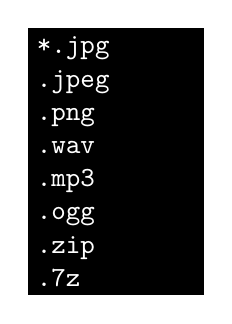
\begin{tikzpicture}
      \node[fill=black,text=white,font=\ttfamily]{
        \parbox{2cm}{
          *.jpg \\
          *.jpeg \\
          *.png \\
          *.wav \\
          *.mp3 \\
          *.ogg \\
          *.zip \\
          *.7z
        }
      };
    \end{tikzpicture}
  \end{center}
\end{frame}